\section{The measurement problem}
\label{sec:measurement}

\begin{figure*}[t]
\centering
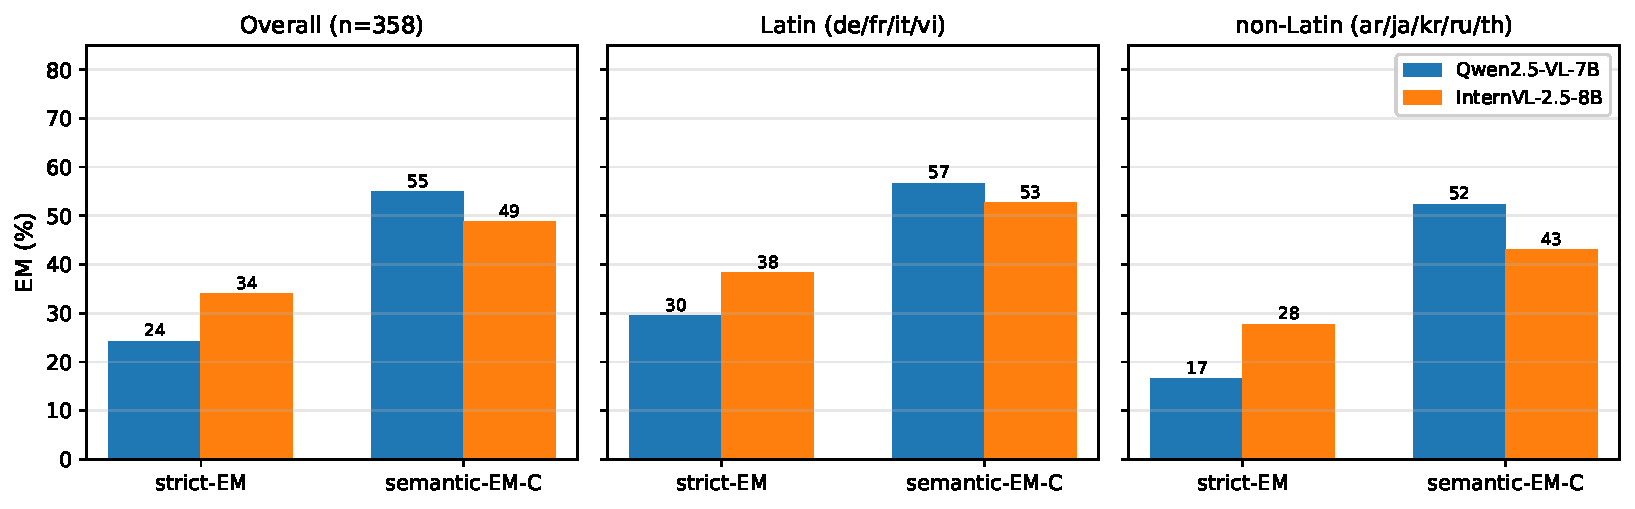
\includegraphics[width=0.95\textwidth]{figures/fig_headline_strict_vs_semantic.pdf}
\caption{Strict-EM vs semantic-EM on 358-row MTVQA held-out for Qwen2.5-VL-7B and InternVL-2.5-8B. Three panels: overall, Latin scripts (de/fr/it/vi), non-Latin scripts (ar/ja/kr/ru/th). InternVL leads under strict-EM in all three panels; Qwen leads under semantic-EM in all three. The metric choice flips the cross-VLM ranking.}
\label{fig:headline}
\end{figure*}

\paragraph{Overall lift and Latin/non-Latin decomposition.}
On the 358-row MTVQA held-out, base Qwen2.5-VL-7B produces 92 strict-EM hits ($25.7\%$), 195 semantic-CORRECT verdicts ($54.5\%$), and 257 \textsc{C+Partial} verdicts ($71.8\%$). Slightly more than half of the model's apparent strict-EM ``failures'' are surface-form-penalised semantically correct answers; aggressive-normalisation EM (NFKC + lowercase + whitespace-collapse) reaches only $35.5\%$, so the remaining $+19$ pp strict$\to$sem-C gap is paraphrase, valid translation, and granularity rather than typography. Table~\ref{tab:script-gap-mtvqa} decomposes the script gap: strict-EM produces a $+13.6$ pp Latin advantage that shrinks to $+4.7$ pp under semantic-CORRECT, an implied \textbf{artifact share}\footnote{We define artifact share as $1 - (g_{\text{semantic}} / g_{\text{strict}})$. A share of $65\%$ means $65\%$ of the strict-EM gap disappears when we credit semantically-equivalent answers.} of $65\%$. Most of what strict-EM measures as a Latin-favourable cross-lingual gap is the model writing non-Latin-script answers in shapes that don't byte-match a single gold answer string. Per-language strict$\to$sem-C lifts are largest on Russian ($+42.1$ pp), Japanese ($+40.3$), Italian ($+35.8$), and Arabic ($+31.4$); these are the languages where the model writes longer, less-byte-aligned answers (per-language table in Appendix~\ref{app:per-language}).

\begin{table}[t]
\centering
\small
\begin{tabular}{lrrr}
\toprule
metric & Latin & non-Latin & gap \\
\midrule
strict-EM       & 31.3\% & 17.7\% & $+13.6$ pp \\
normalized-EM   & 33.6\% & 22.4\% & $+11.2$ pp \\
semantic-EM-C   & 56.4\% & 51.7\% & $+4.7$ pp \\
semantic-EM-C+P & 75.8\% & 66.0\% & $+9.8$ pp \\
\bottomrule
\end{tabular}
\caption{Script-level decomposition of Qwen2.5-VL-7B on 358-row MTVQA held-out (Latin: de/fr/it/vi, $n=211$; non-Latin: ar/ja/kr/ru/th, $n=147$). Strict-EM gap $+13.6$ pp; semantic-CORRECT only $+4.7$ pp; \textbf{artifact share $=65\%$}.}
\label{tab:script-gap-mtvqa}
\end{table}

\paragraph{Population-level replication and implication.}
We re-judge full Qwen2.5-VL-7B base predictions on the entire 9-language MTVQA val split ($n=2203$; $2163$ rows received clean verdicts after retry exhaustion). Population aggregates: strict-EM $\mathbf{29.2\%}$, semantic-EM-C $\mathbf{60.6\%}$, semantic-EM-C+P $\mathbf{75.7\%}$; Latin/non-Latin script gap is strict $+20.3$ pp $\to$ semantic-C $+13.4$ pp, an \textbf{artifact share of $34\%$} --- smaller than the $65\%$ on the held-out (which enriches for high-artifact-share failures by construction) but still substantial, bootstrap-significant, and consistent in direction. Strict-EM cross-lingual evaluation reads three signals simultaneously: (a) capability, (b) output-style alignment to a single gold string, (c) per-language ambiguity in what a ``correct'' answer means. The next two sections show that signals (b) and (c) are not random noise: they are biased differently by VLM architecture (\S\ref{sec:inversion}) and differently by intervention (\S\ref{sec:interventions}).
